\section{Equations of motion for grains with radiation and gas drag}
\label{sec:equat-moti-grains}

\begin{figure}
  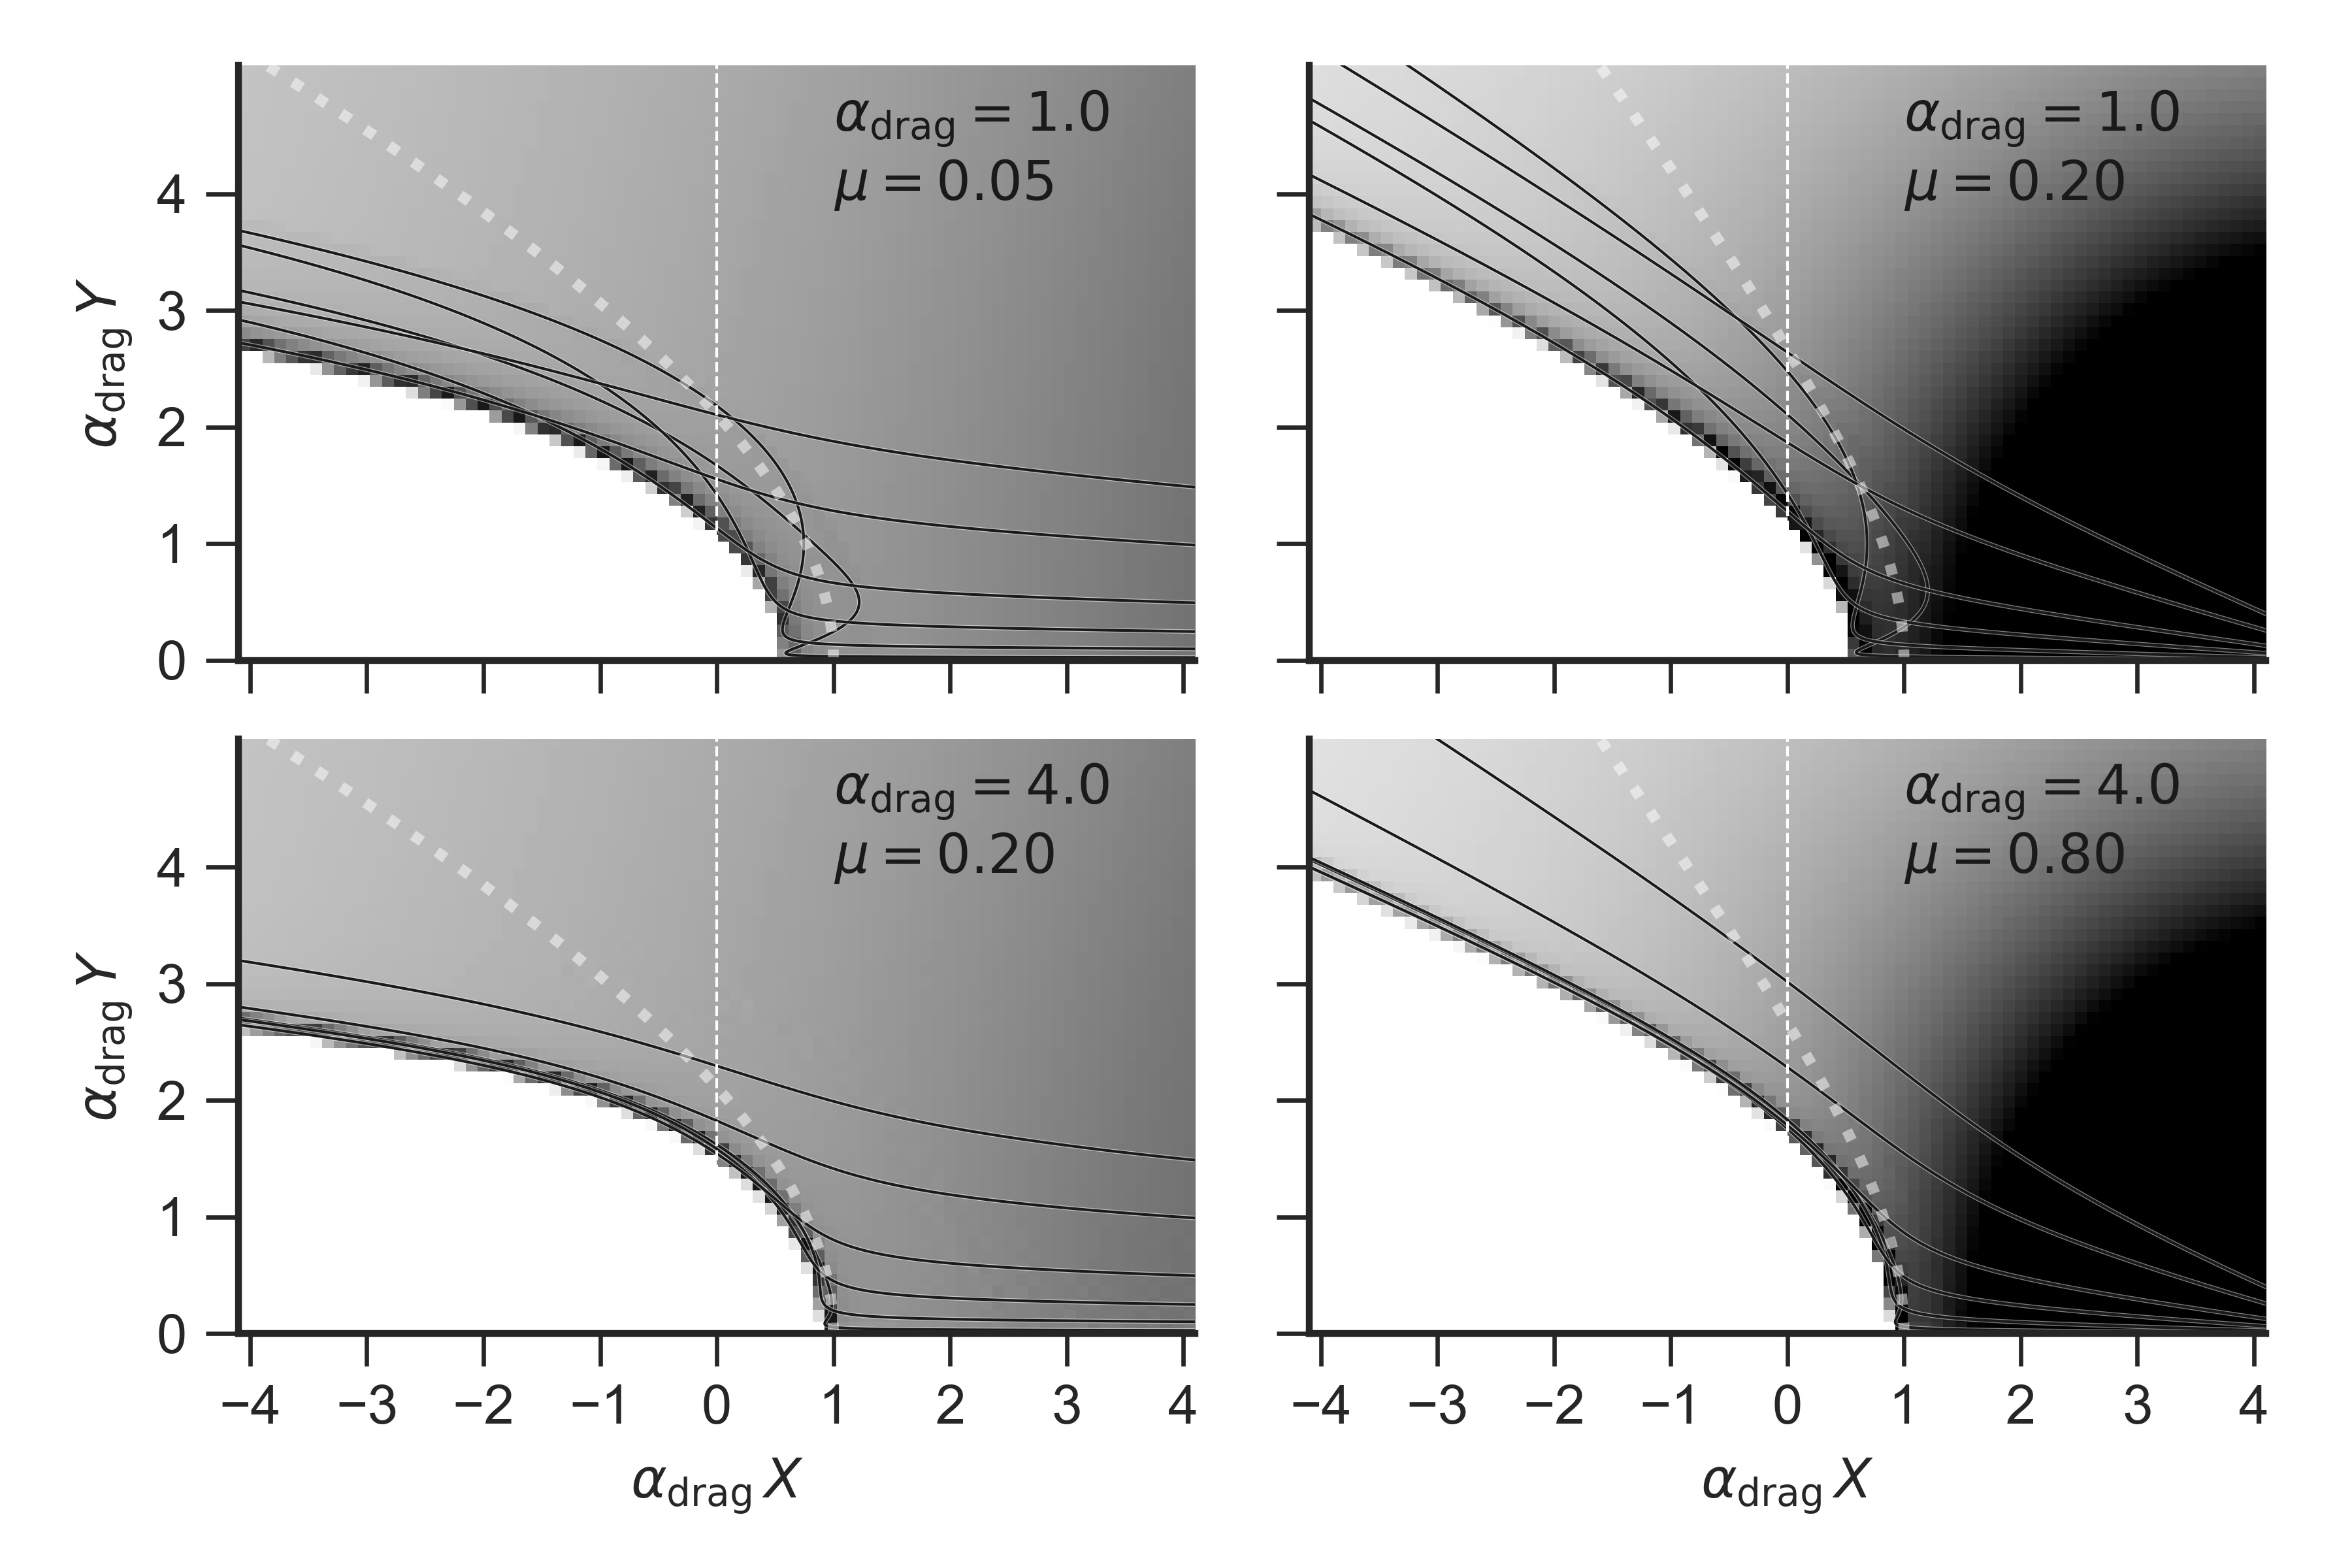
\includegraphics[width=\linewidth]{figs/dust-couple-div-stream}
  \caption{Divergent dragoids}
  \label{fig:divergent-dragoids}
\end{figure}

To find the dust grain trajectories \(R\grain(\theta)\) in the presence of
radiation and drag forces (\S~\ref{sec:bow-wave-drag}), we numerically
integrate the equations of motion. We define dimensionless cylindrical
polar coordinates,
\begin{equation}
  \label{eq:dust-XY}
  (X, Y) = \left(\frac{R\grain(\theta) \cos\theta } {R_0}, \ 
    \frac{R\grain(\theta) \sin\theta } {R_0}\right)
  \ ,
\end{equation}
and dust grain velocities,
\begin{equation}
  \label{eq:dust-UV}
  (U, V) = \left( \frac{\bm{v}\grain \cdot \uvec{x}} {v_\infty}, \ 
  \frac{\bm{v}\grain \cdot \uvec{y}} {v_\infty}\right) \ ,
\end{equation}
where \(\uvec{x}\) and \(\uvec{y}\) are unit vectors along the \(X\)
and \(Y\) axes (parallel and perpendicular, respectively, to the
symmetry axis).  The grain equation of motion then follows from
equations~(\ref{eq:dust-rad-force}, \ref{eq:dust-r0},
\ref{eq:dust-fdrag}--\ref{eq:dust-alpha}) as the following set of
coupled differential equations:
\begin{gather}
  \label{eq:dust-motion}
  \begin{aligned}
    \frac{d X}{d t} &= U \quad\quad
    \frac{d Y}{d t} = V \\
    \frac{d U}{d t} &= \frac12 \left[  
      X \left(X^2 + Y^2\right)^{-3/2} - \alpha\drag^2 D_1 \left(U - U_1\right)
    \right] \\
    \frac{d V}{d t} &= \frac12 \left[  
      Y \left(X^2 + Y^2\right)^{-3/2} - \alpha\drag^2 D_1 \left(V - V_1\right)
    \right] \ ,
  \end{aligned}
\end{gather}
where \((U_1, V_1)\) are the components of the gas velocity (assumed
fixed), given by
\begin{equation}
  \label{eq:dust-gas-velocities}
  (U_1, V_1) = 
  \begin{cases}
    \text{parallel stream} & (-1, 0)\\
    \text{divergent stream} &
    \left( \dfrac{X - \mu^{-1}}{R_1},\ \dfrac{Y}{R_1}\right) \ ,
  \end{cases}
\end{equation}
where
\begin{equation}
  \label{eq:dust-R1}
  R_1 = \left( \bigl(X - \mu^{-1}\bigr)^2 + Y^2 \right)^{1/2}
\end{equation}
is the distance from the second source, located at
\((X, Y) = (\mu^{-1}, 0)\).  The dimensionless gas density, \(D_1\),
normalized by the value at \((X, Y) = (1, 0)\), is
\begin{equation}
  \label{eq:dust-gas-density}
  D_1 = 
  \begin{cases}
    \text{parallel stream} & 1\\
    \text{divergent stream} & \dfrac{\bigl(\mu^{-1} - 1\bigr)^2} {R_1^{2}} \ .
  \end{cases}
\end{equation}

Equations~\eqref{eq:dust-motion} are integrated using the python
wrapper \texttt{scipy.integrate.odeint} to the Fortran ODEPACK library
\citep{Hindmarsh:1983a, Jones:2001a}, with results shown in
Figure~\ref{fig:dust-wave-coupling} for parallel-stream cases and
Figure~\ref{fig:divergent-dragoids} for divergent-stream cases. 

%%% Local Variables:
%%% mode: latex
%%% TeX-master: "dusty-bow-wave"
%%% End:
